\documentclass[]{article}
\usepackage{lmodern}
\usepackage{amssymb,amsmath}
\usepackage{ifxetex,ifluatex}
\usepackage{fixltx2e} % provides \textsubscript
\ifnum 0\ifxetex 1\fi\ifluatex 1\fi=0 % if pdftex
  \usepackage[T1]{fontenc}
  \usepackage[utf8]{inputenc}
\else % if luatex or xelatex
  \ifxetex
    \usepackage{mathspec}
  \else
    \usepackage{fontspec}
  \fi
  \defaultfontfeatures{Ligatures=TeX,Scale=MatchLowercase}
\fi
% use upquote if available, for straight quotes in verbatim environments
\IfFileExists{upquote.sty}{\usepackage{upquote}}{}
% use microtype if available
\IfFileExists{microtype.sty}{%
\usepackage{microtype}
\UseMicrotypeSet[protrusion]{basicmath} % disable protrusion for tt fonts
}{}
\usepackage[margin=1in]{geometry}
\usepackage{hyperref}
\hypersetup{unicode=true,
            pdftitle={Consumer attitude towards fish sauce products},
            pdfauthor={Xuan Pham},
            pdfborder={0 0 0},
            breaklinks=true}
\urlstyle{same}  % don't use monospace font for urls
\usepackage{natbib}
\bibliographystyle{plainnat}
\usepackage{graphicx}
% grffile has become a legacy package: https://ctan.org/pkg/grffile
\IfFileExists{grffile.sty}{%
\usepackage{grffile}
}{}
\makeatletter
\def\maxwidth{\ifdim\Gin@nat@width>\linewidth\linewidth\else\Gin@nat@width\fi}
\def\maxheight{\ifdim\Gin@nat@height>\textheight\textheight\else\Gin@nat@height\fi}
\makeatother
% Scale images if necessary, so that they will not overflow the page
% margins by default, and it is still possible to overwrite the defaults
% using explicit options in \includegraphics[width, height, ...]{}
\setkeys{Gin}{width=\maxwidth,height=\maxheight,keepaspectratio}
\IfFileExists{parskip.sty}{%
\usepackage{parskip}
}{% else
\setlength{\parindent}{0pt}
\setlength{\parskip}{6pt plus 2pt minus 1pt}
}
\setlength{\emergencystretch}{3em}  % prevent overfull lines
\providecommand{\tightlist}{%
  \setlength{\itemsep}{0pt}\setlength{\parskip}{0pt}}
\setcounter{secnumdepth}{0}
% Redefines (sub)paragraphs to behave more like sections
\ifx\paragraph\undefined\else
\let\oldparagraph\paragraph
\renewcommand{\paragraph}[1]{\oldparagraph{#1}\mbox{}}
\fi
\ifx\subparagraph\undefined\else
\let\oldsubparagraph\subparagraph
\renewcommand{\subparagraph}[1]{\oldsubparagraph{#1}\mbox{}}
\fi

%%% Use protect on footnotes to avoid problems with footnotes in titles
\let\rmarkdownfootnote\footnote%
\def\footnote{\protect\rmarkdownfootnote}

%%% Change title format to be more compact
\usepackage{titling}

% Create subtitle command for use in maketitle
\providecommand{\subtitle}[1]{
  \posttitle{
    \begin{center}\large#1\end{center}
    }
}

\setlength{\droptitle}{-2em}

  \title{Consumer attitude towards fish sauce products}
    \pretitle{\vspace{\droptitle}\centering\huge}
  \posttitle{\par}
    \author{Xuan Pham}
    \preauthor{\centering\large\emph}
  \postauthor{\par}
      \predate{\centering\large\emph}
  \postdate{\par}
    \date{12/17/2019}

\usepackage{booktabs}
\usepackage{longtable}
\usepackage{array}
\usepackage{multirow}
\usepackage{wrapfig}
\usepackage{float}
\usepackage{colortbl}
\usepackage{pdflscape}
\usepackage{tabu}
\usepackage{threeparttable}
\usepackage{threeparttablex}
\usepackage[normalem]{ulem}
\usepackage{makecell}
\usepackage{xcolor}

\begin{document}
\maketitle

{
\setcounter{tocdepth}{2}
\tableofcontents
}
\hypertarget{setting-up-the-working-environment}{%
\section{1. Setting up the working
environment}\label{setting-up-the-working-environment}}

\hypertarget{import-data}{%
\section{2. Import data}\label{import-data}}

\hypertarget{sample-structure-understanding}{%
\section{3. Sample structure
understanding}\label{sample-structure-understanding}}

\hypertarget{categorical-variables}{%
\subsection{3.1 Categorical variables}\label{categorical-variables}}

Majority of respondents are female in their 20s (20-24 yo), obtained
University degree, having full-time jobs and originally from the South.

\hypertarget{sample-structure-table-summary}{%
\subsubsection{3.1.1 Sample structure table
summary}\label{sample-structure-table-summary}}

\textbackslash begin\{tabular\}\{llrr\} \toprule \textbf{Variable} \&
\textbf{Level} \& \textbf{No. of respondents} \&
\textbackslash textbf\{\% Respondents\}\textbackslash{} \midrule Age
range \& 20-24 yo \& 173 \& 57.67\textbackslash{} Age range \& Above 35
yo \& 71 \& 23.67\textbackslash{} Age range \& 25-35 yo \& 56 \&
18.67\textbackslash{} Education level \& University \& 267 \&
89.00\textbackslash{} Education level \& High school \& 31 \&
10.33\textbackslash{} \addlinespace Education level \& Below high school
\& 2 \& 0.67\textbackslash{} Gender \& Female \& 199 \&
66.33\textbackslash{} Gender \& Male \& 101 \& 33.67\textbackslash{} Job
\& Full-time \& 155 \& 51.67\textbackslash{} Job \& Student \& 103 \&
34.33\textbackslash{} \addlinespace Job \& Part-time \& 33 \&
11.00\textbackslash{} Job \& Housework \& 9 \& 3.00\textbackslash{}
Native village \& South \& 195 \& 65.00\textbackslash{} Native village
\& Central \& 66 \& 22.00\textbackslash{} Native village \& North \& 39
\& 13.00\textbackslash{} \bottomrule \textbackslash end\{tabular\}

\hypertarget{sample-structure-plot}{%
\subsubsection{3.1.2 Sample structure
plot}\label{sample-structure-plot}}

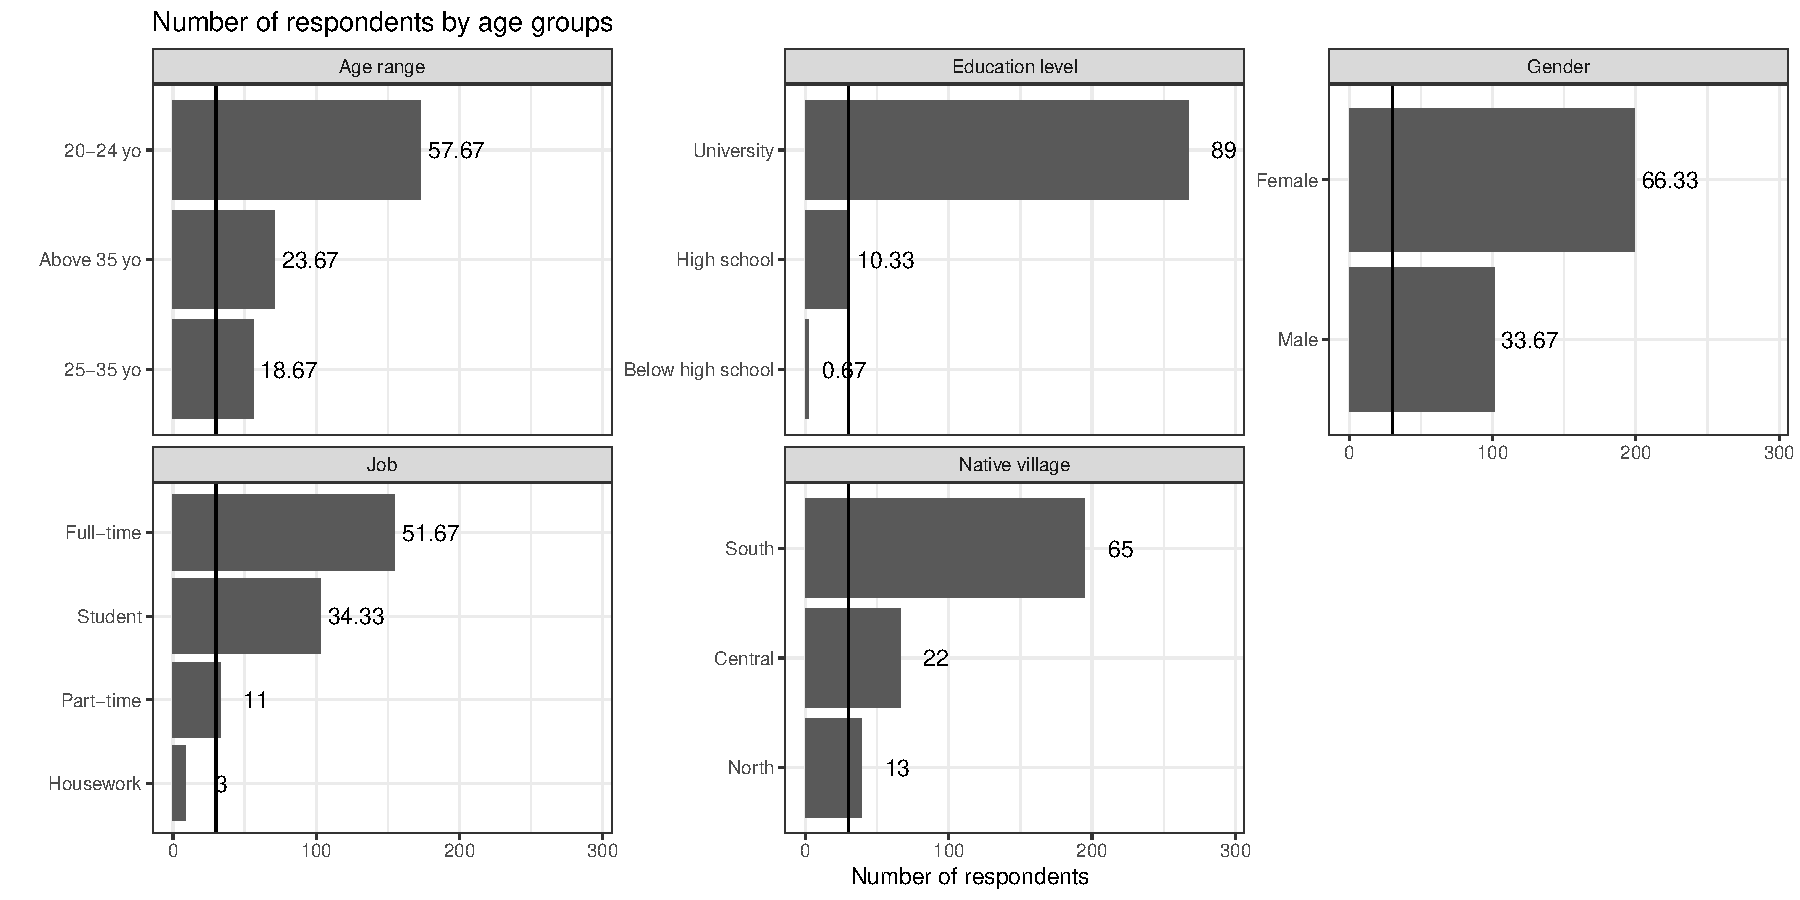
\includegraphics{Consumer-attitude-towards-fish-sauce-products_files/figure-latex/unnamed-chunk-6-1.pdf}

\hypertarget{continuous-variables}{%
\subsection{3.2 Continuous variables}\label{continuous-variables}}

Respondent age is not normally distributed. 1/3 respondents are 22 years
old.

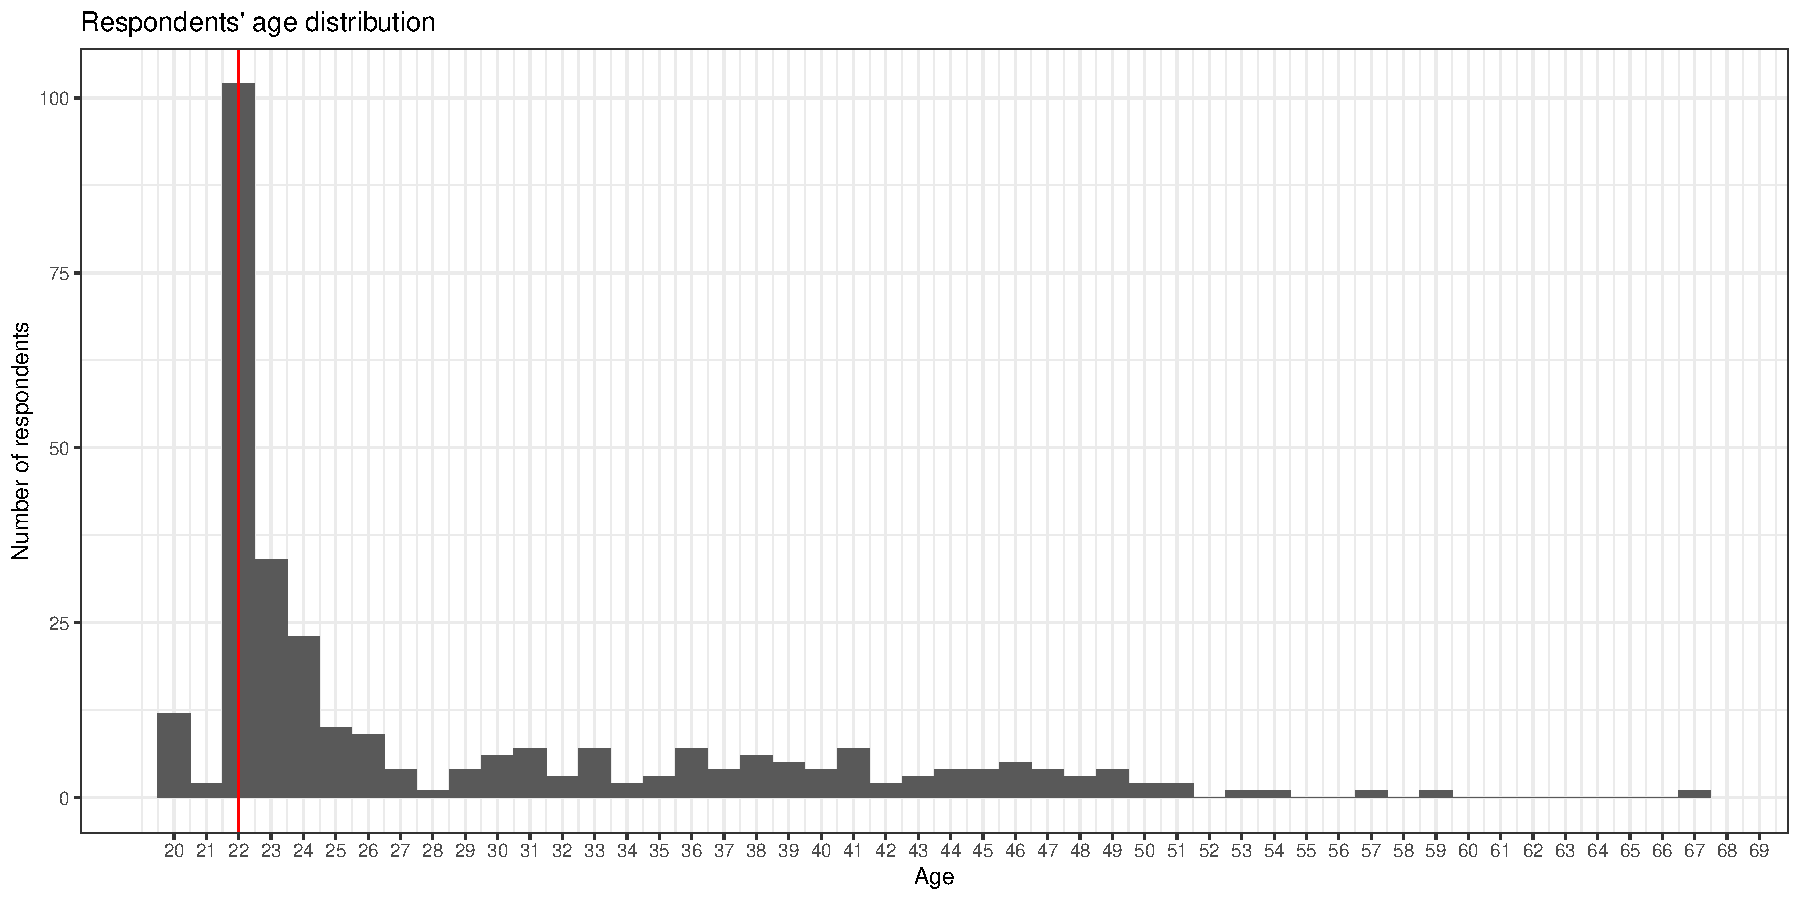
\includegraphics{Consumer-attitude-towards-fish-sauce-products_files/figure-latex/unnamed-chunk-7-1.pdf}

\hypertarget{continuous-vs.-categorical-variables}{%
\subsection{3.3 Continuous vs.~categorical
variables}\label{continuous-vs.-categorical-variables}}

Female respondents age is extremely right skewed.
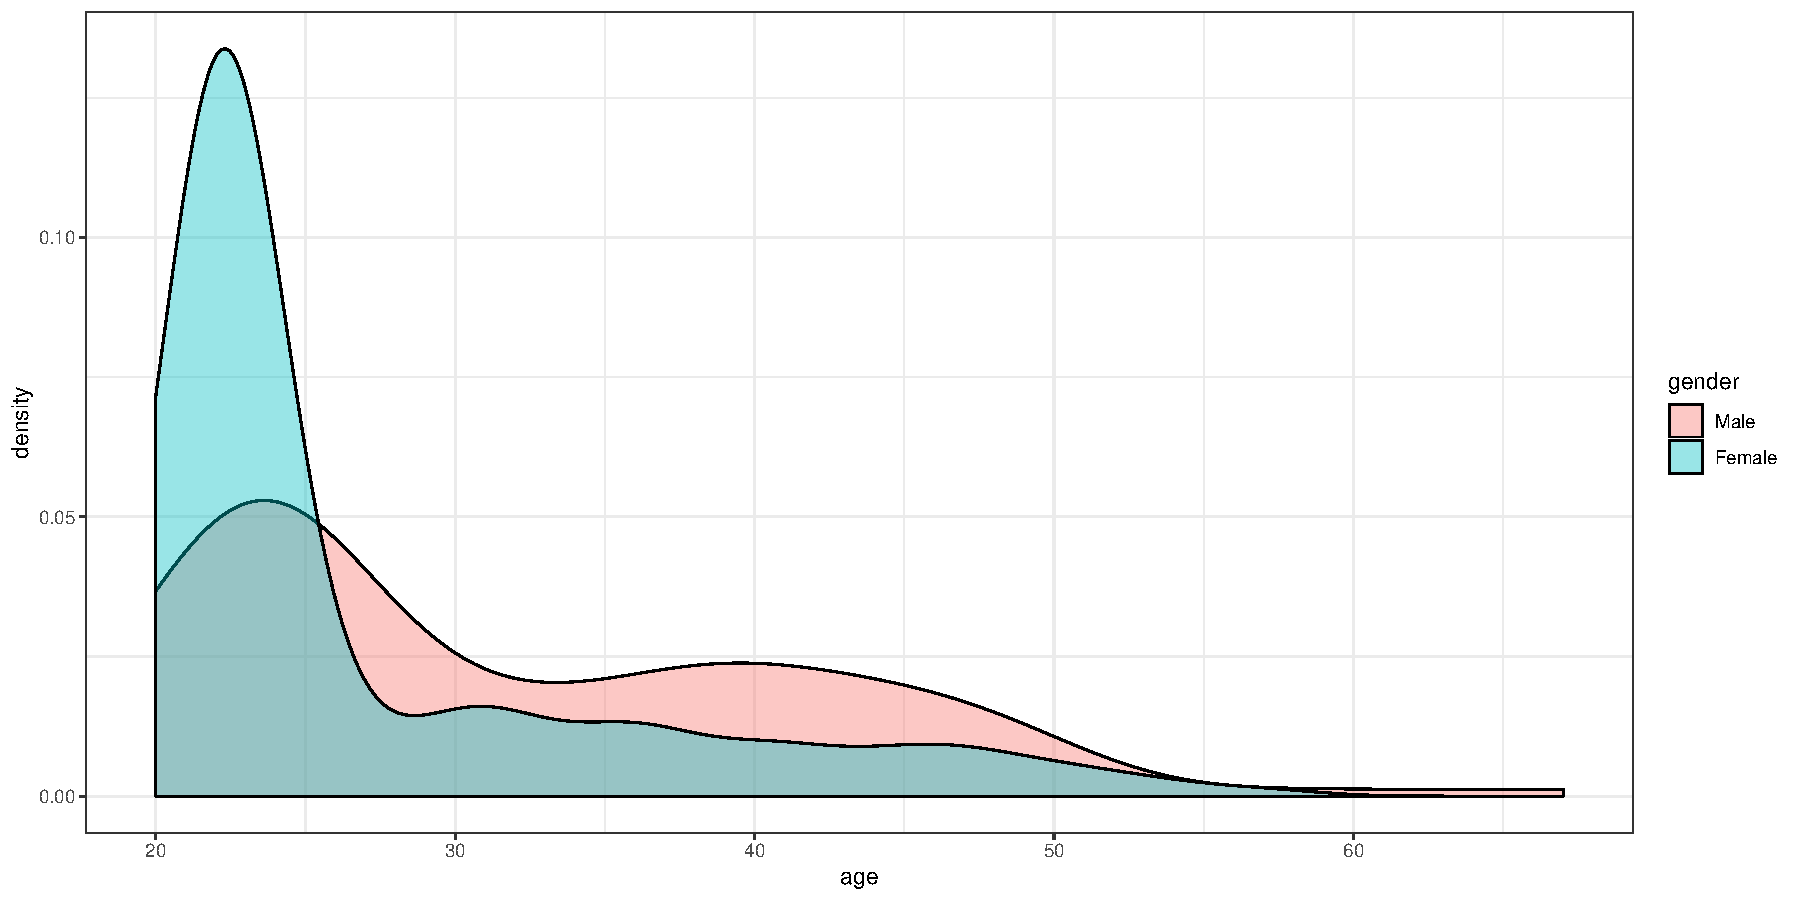
\includegraphics{Consumer-attitude-towards-fish-sauce-products_files/figure-latex/unnamed-chunk-8-1.pdf}

Age distributions of those who are from the South and Central are wider
spread than the North group.
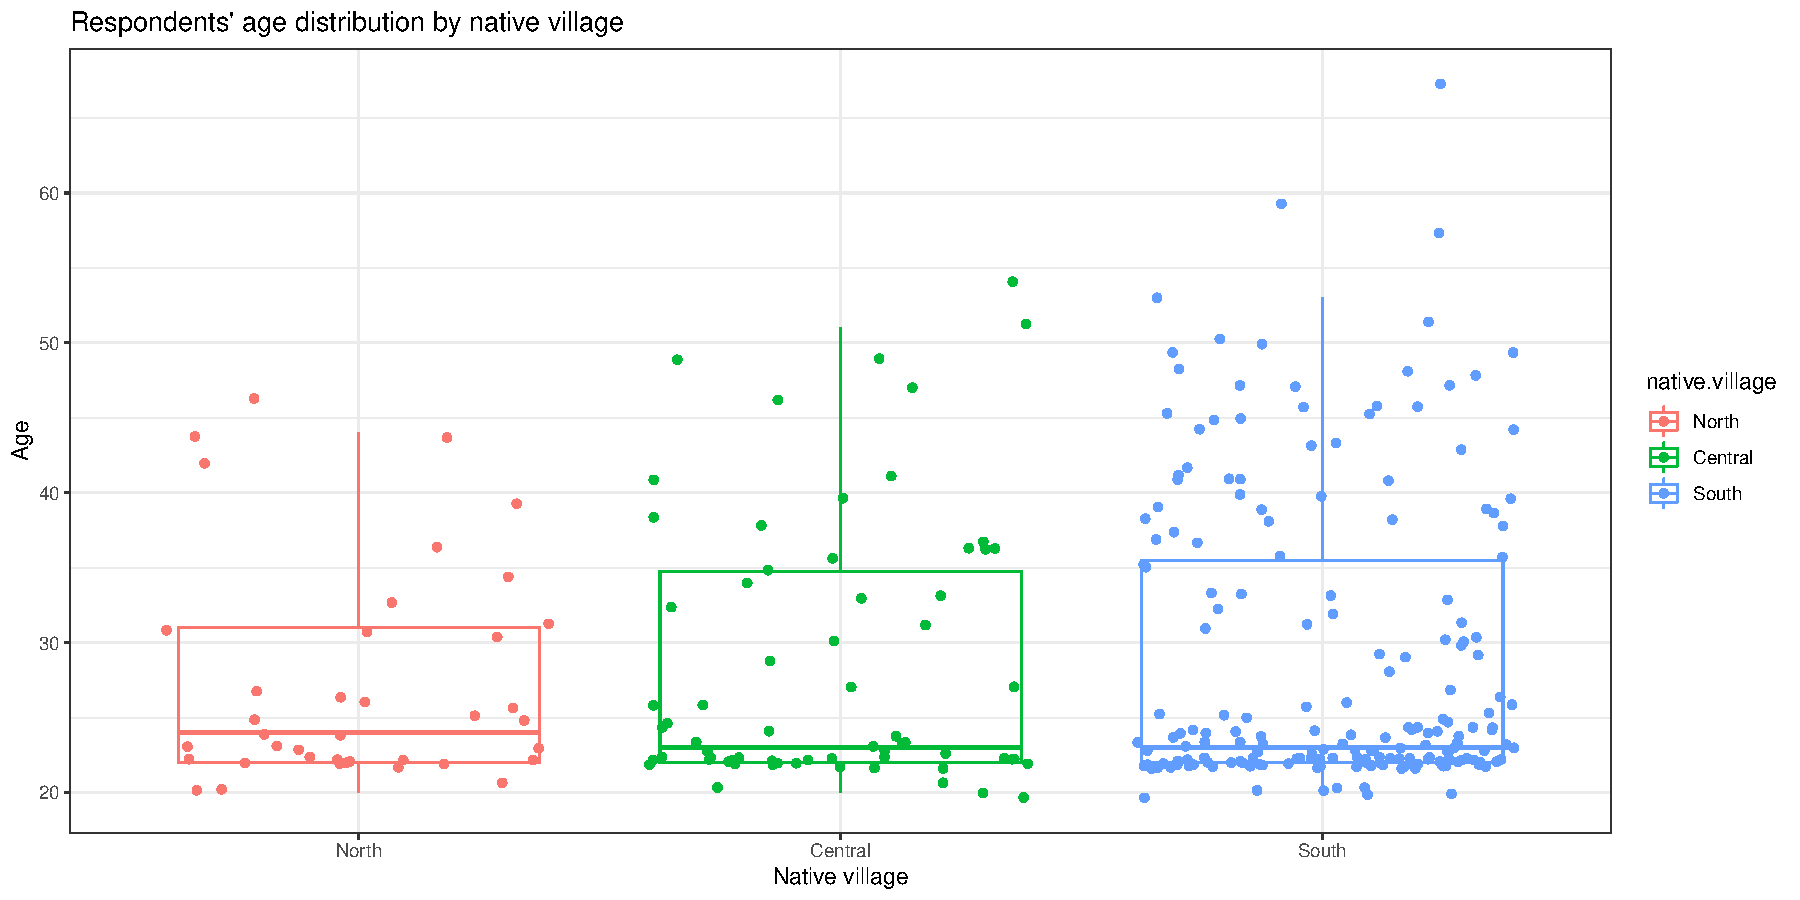
\includegraphics{Consumer-attitude-towards-fish-sauce-products_files/figure-latex/unnamed-chunk-9-1.pdf}

\hypertarget{data-cleaning}{%
\section{4. Data cleaning}\label{data-cleaning}}

Coding error is spotted! Each variable in brand section should have two
levels only. Khai hoan brand has 4 levels.

\begin{verbatim}
      ID                phu.quoc        phan.thiet     nam.ngu   
 Length:300         kh.pq   :256   kh.pt     :282   kh.nn  :150  
 Class :character   phu.quoc: 44   phan.thiet: 18   nam.ngu:150  
 Mode  :character                                                
                                                                 
     hanh.phuc        thanh.phong      de.nhi       chinsu       co.hau   
 hanh.phuc: 19   kh.tp      :299   de.nhi : 25   chinsu: 56   co.hau:  1  
 kh.hp    :281   thanh.phong:  1   kh.dnhi:275   kh.cs :244   kh.ch :299  
                                                                          
                                                                          
      hung.thinh     ba.mien        cholimex       nha.trang        hong.thanh 
 hung.thinh: 39   ba.mien:  2   cholimex:  3   kh.nt    :292   hong.thanh:  4  
 kh.ht     :261   kh.bm  :298   kh.cho  :297   nha.trang:  8   kh.hthanh :296  
                                                                               
                                                                               
     khai.hoan        thien.huong      tu.tuyet        lien.thanh 
 k        :  7   kh.th      :298   kh.tt   :298   kh.lt     :283  
 kh.kh    :259   thien.huong:  2   tu.tuyet:  2   lien.thanh: 17  
 khai.hoan:  5                                                    
 NA's     : 29                                                    
\end{verbatim}

Nam Ngu is the most popular brand and almost triple the second player -
Chinsu in terms of the number of responses.

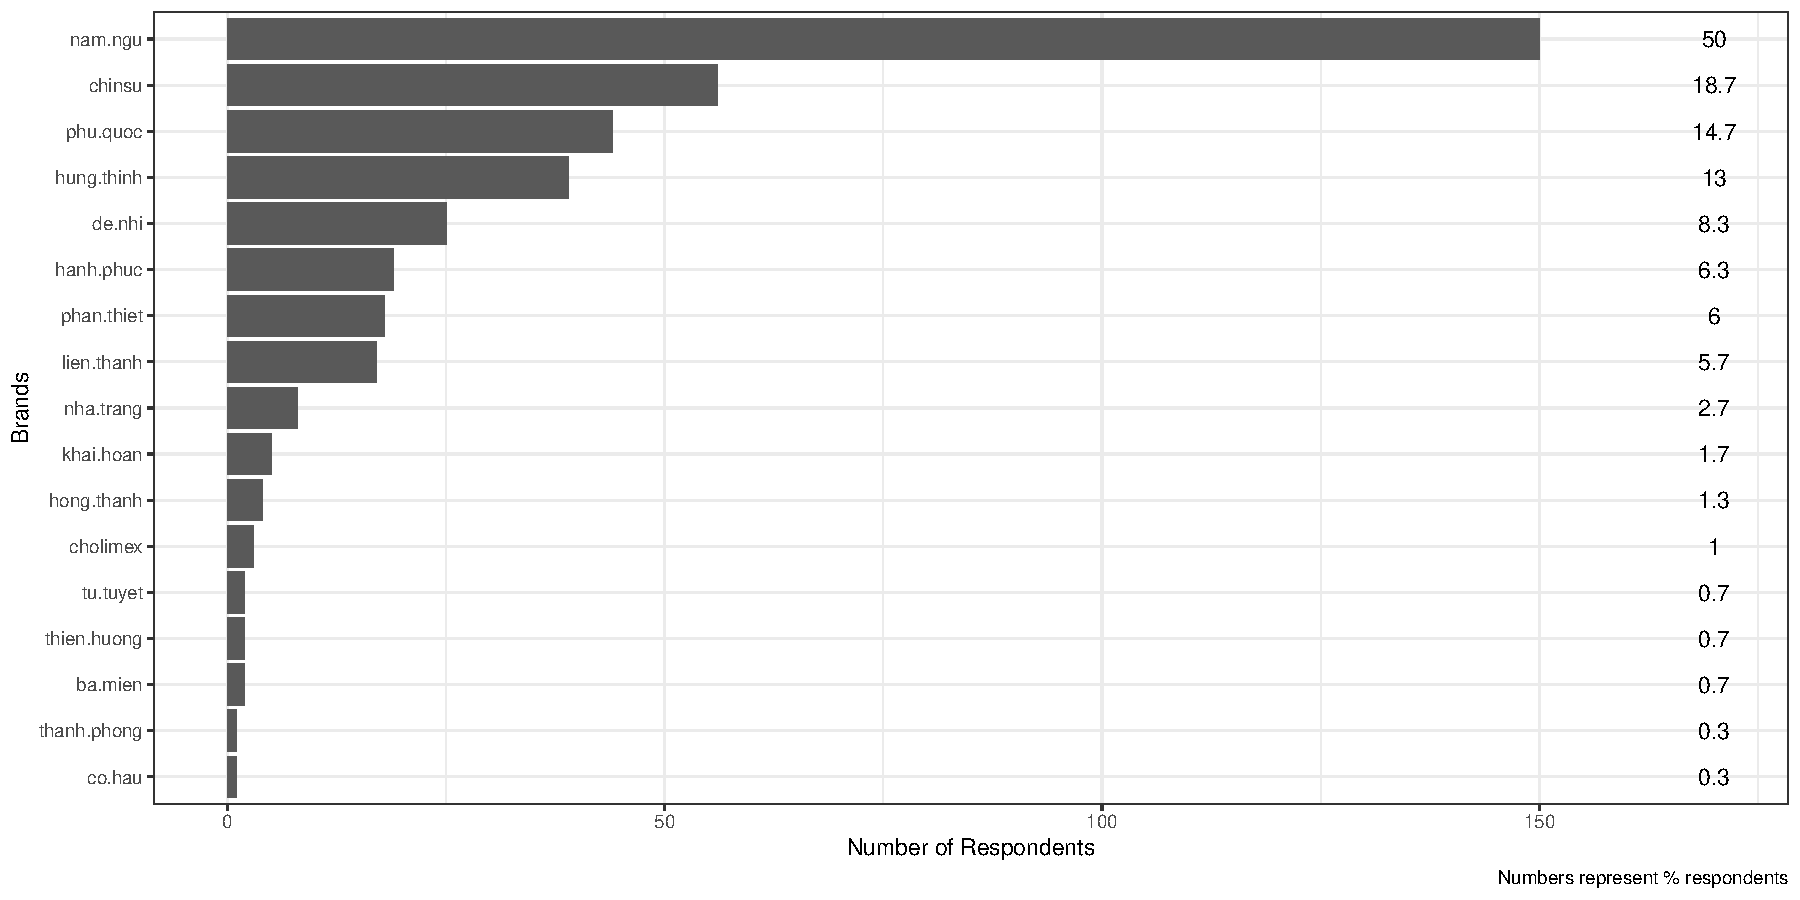
\includegraphics{Consumer-attitude-towards-fish-sauce-products_files/figure-latex/unnamed-chunk-11-1.pdf}

There are few respondents gave more than required number of responses
(maximum is 2).

\begin{tabular}{lllllr}
\toprule
\textbf{Respondent ID} & \textbf{Brand 1} & \textbf{Brand 2} & \textbf{Brand 3} & \textbf{Brand 4} & \textbf{Number of brands declared}\\
\midrule
KS2_29 & phu.quoc & phan.thiet & nam.ngu & hung.thinh & 4\\
KS2_111 & phu.quoc & nam.ngu & nha.trang & NA & 3\\
KS2_130 & nam.ngu & chinsu & cholimex & NA & 3\\
KS2_181 & hanh.phuc & chinsu & hung.thinh & NA & 3\\
KS2_224 & phu.quoc & nam.ngu & lien.thanh & NA & 3\\
\addlinespace
KS2_255 & hung.thinh & tu.tuyet & lien.thanh & NA & 3\\
KS2_109 & phu.quoc & hung.thinh & NA & NA & 2\\
KS2_110 & hung.thinh & cholimex & NA & NA & 2\\
KS2_113 & de.nhi & hung.thinh & NA & NA & 2\\
KS2_115 & nam.ngu & de.nhi & NA & NA & 2\\
\bottomrule
\end{tabular}

\hypertarget{data-exploration}{%
\section{5. Data exploration}\label{data-exploration}}

\hypertarget{key-influencing-factors}{%
\subsection{5.1 Key influencing factors}\label{key-influencing-factors}}

\begin{tabular}{rrrrrr}
\toprule
\textbf{Health} & \textbf{Sensory} & \textbf{Tradition} & \textbf{Quality} & \textbf{Price} & \textbf{Convenience}\\
\midrule
3.95 & 4.09 & 3.98 & 4.16 & 4 & 4.08\\
\bottomrule
\end{tabular}

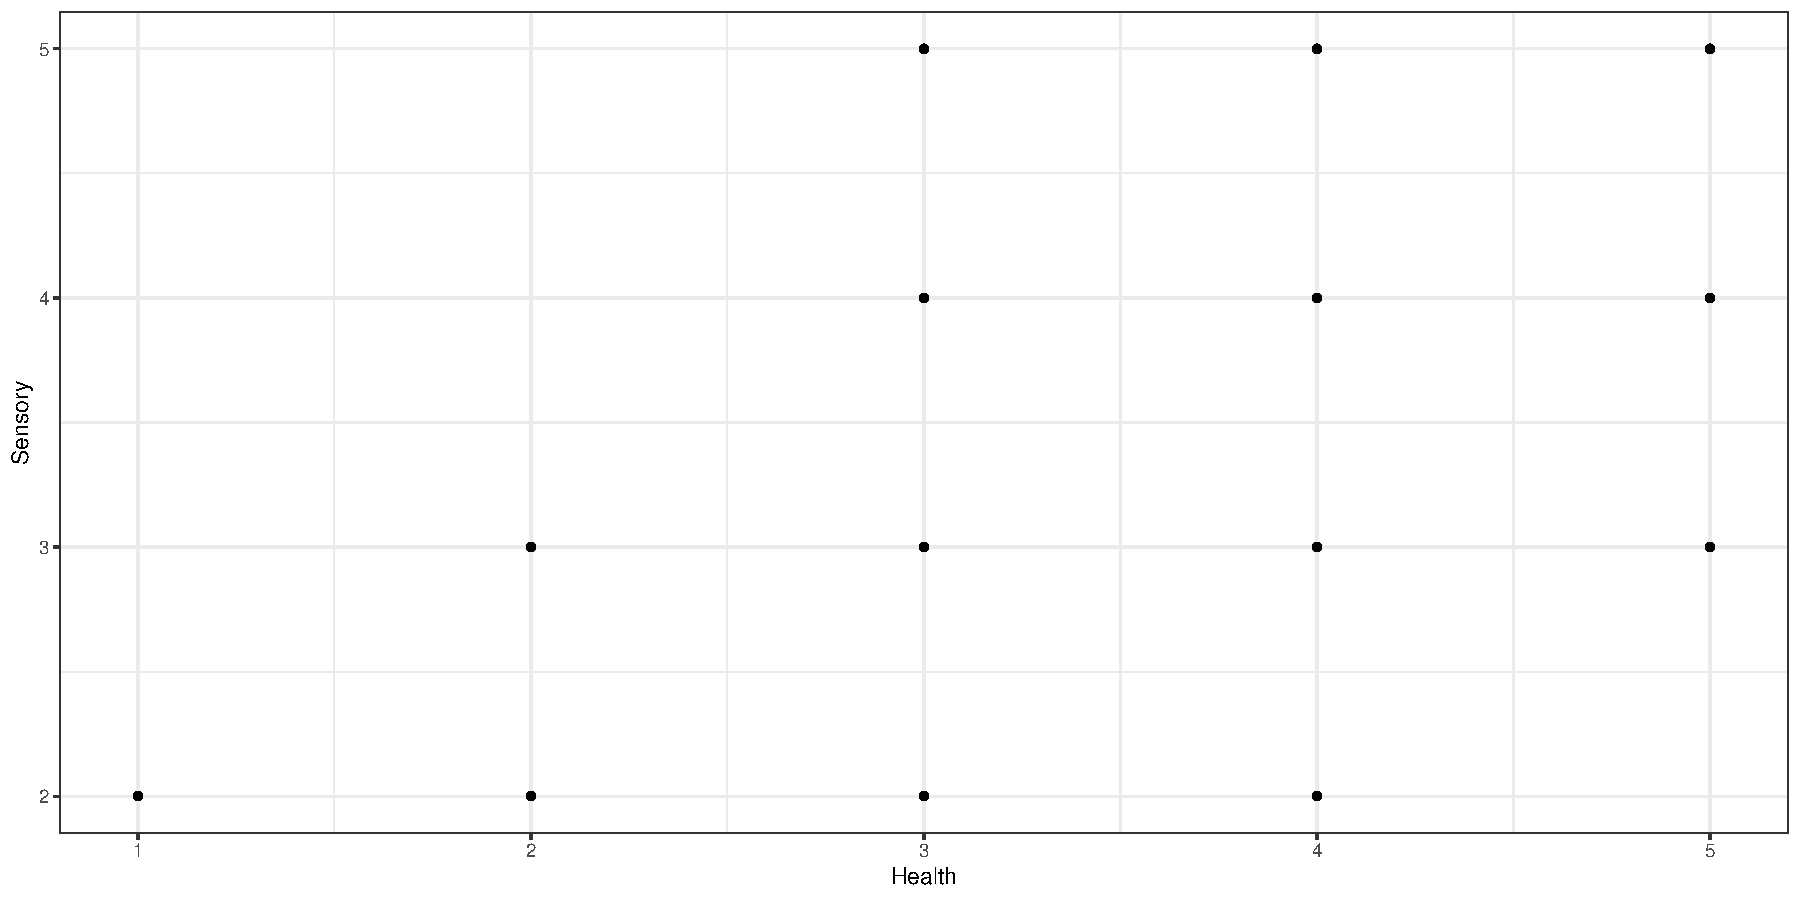
\includegraphics{Consumer-attitude-towards-fish-sauce-products_files/figure-latex/unnamed-chunk-13-1.pdf}
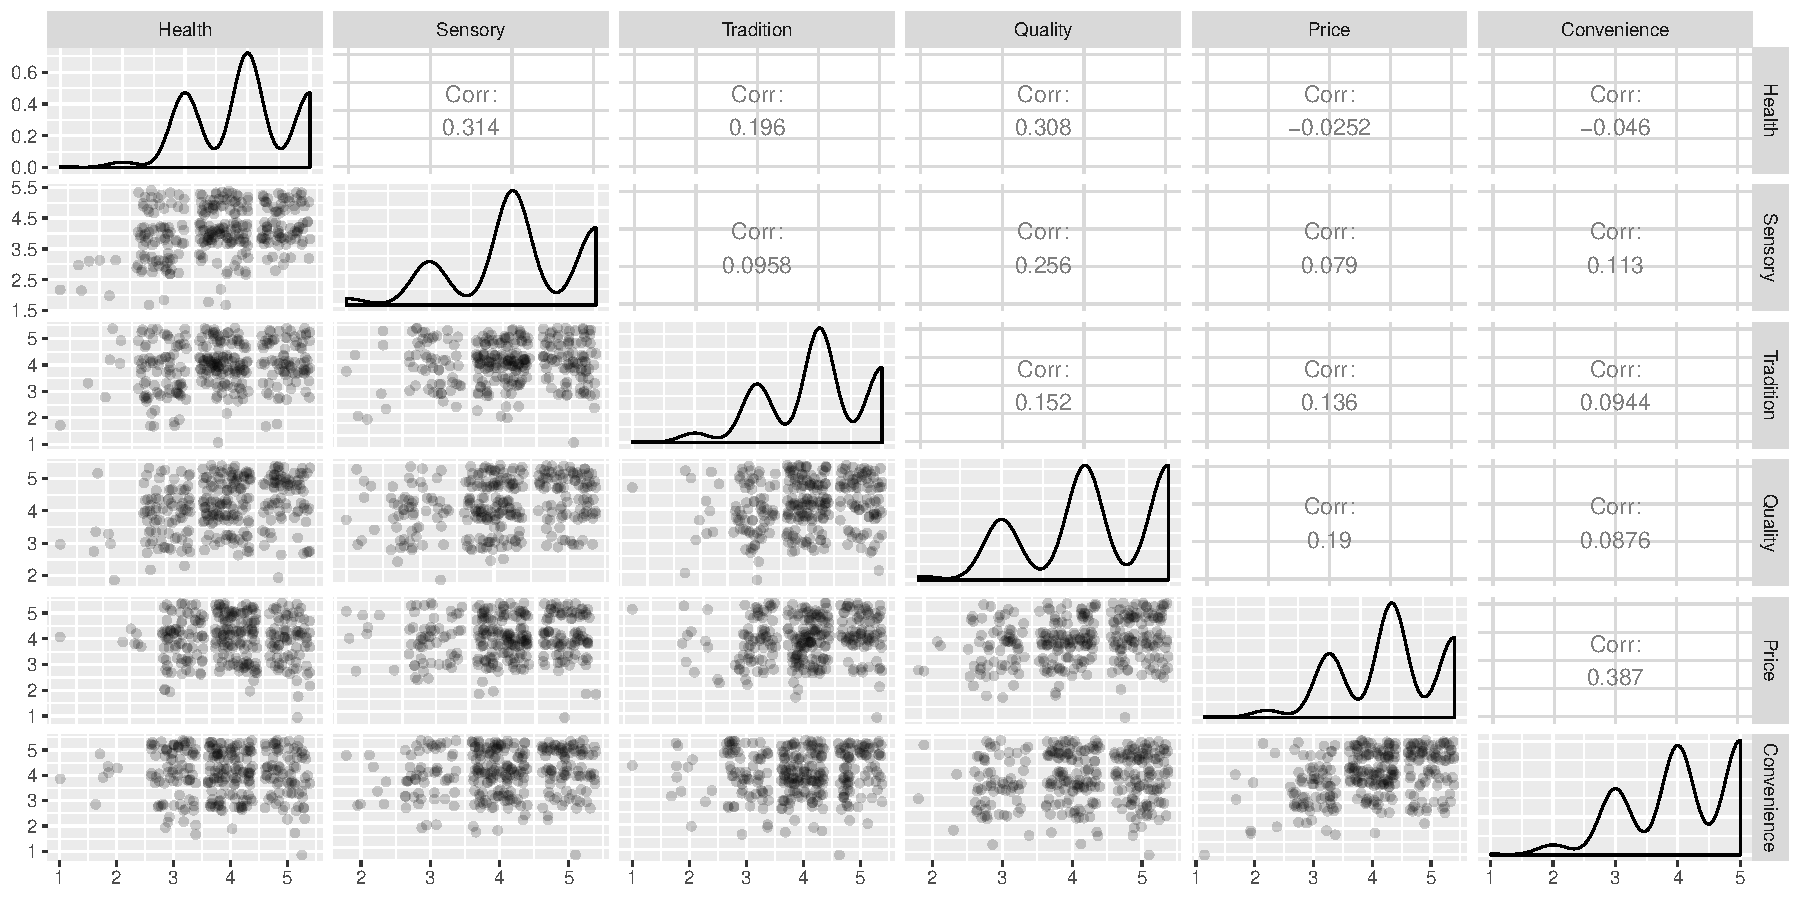
\includegraphics{Consumer-attitude-towards-fish-sauce-products_files/figure-latex/unnamed-chunk-13-2.pdf}
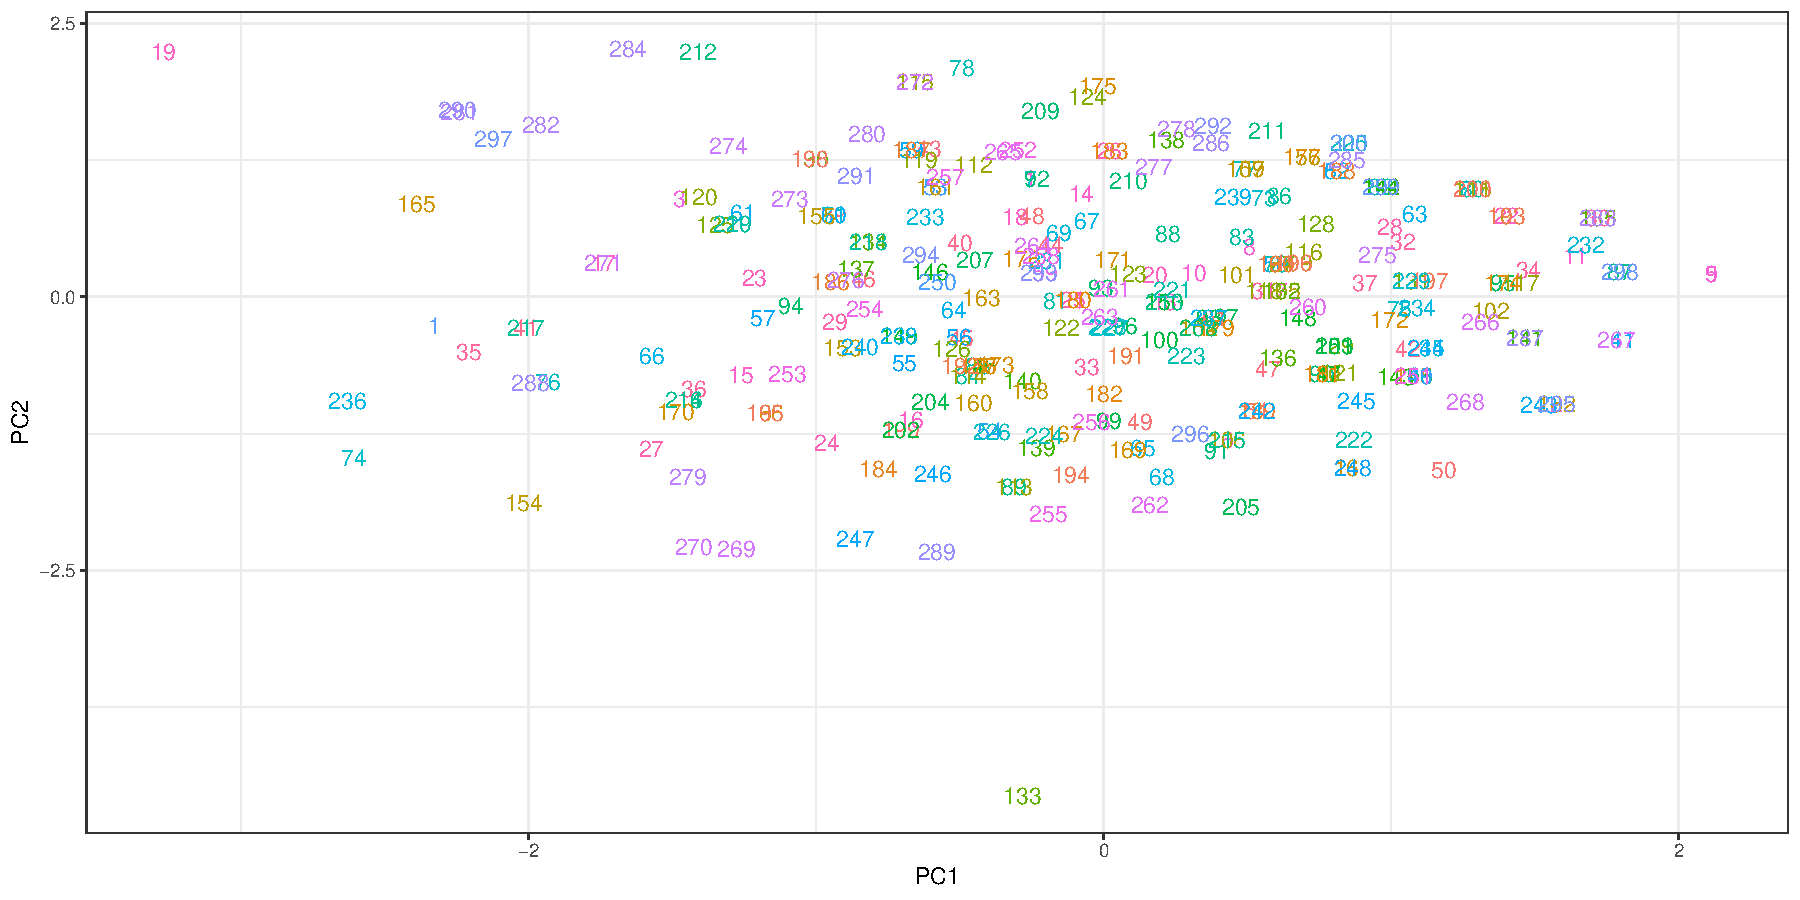
\includegraphics{Consumer-attitude-towards-fish-sauce-products_files/figure-latex/unnamed-chunk-13-3.pdf}

\begin{tabular}{rrrrrr}
\toprule
\textbf{Health} & \textbf{Sensory} & \textbf{Tradition} & \textbf{Quality} & \textbf{Price} & \textbf{Convenience}\\
\midrule
1 & 2 & 2 & 3 & 4 & 4\\
\bottomrule
\end{tabular}

\begin{tabular}{rrrrrr}
\toprule
\textbf{Health} & \textbf{Sensory} & \textbf{Tradition} & \textbf{Quality} & \textbf{Price} & \textbf{Convenience}\\
\midrule
5 & 5 & 5 & 5 & 1 & 1\\
\bottomrule
\end{tabular}

\hypertarget{important-factors}{%
\subsection{5.2 Important factors}\label{important-factors}}

\begin{tabular}{ll}
\toprule
\textbf{Factors} & \textbf{Value}\\
\midrule
\addlinespace[0.3em]
\multicolumn{2}{l}{\textbf{Convenience}}\\
\hspace{1em}Can be bought in shops close to where I live or work & \textcolor{black}{3.85}\\
\hspace{1em}Is easily available in shops and supermarkets & \textcolor[HTML]{1e90ff}{\textbf{4.04}}\\
\hspace{1em}Is easy to prepare & \textcolor{black}{3.83}\\
\hspace{1em}Takes no time to prepare & \textcolor{black}{3.91}\\
\addlinespace[0.3em]
\multicolumn{2}{l}{\textbf{Health}}\\
\hspace{1em}Contains lots of protein, vitamins, omega-3, iron and lysine & \textcolor{black}{3.9}\\
\hspace{1em}Eating with fish sauce will help us eat more, thus providing more active energy & \textcolor{black}{3.68}\\
\hspace{1em}Keeps me healthy & \textcolor{black}{3.82}\\
\addlinespace[0.3em]
\multicolumn{2}{l}{\textbf{Price}}\\
\hspace{1em}Is cheap & \textcolor{black}{3.25}\\
\hspace{1em}Is good value for money & \textcolor[HTML]{1e90ff}{\textbf{4.02}}\\
\hspace{1em}Is not expensive & \textcolor{black}{3.65}\\
\addlinespace[0.3em]
\multicolumn{2}{l}{\textbf{Quality and safety}}\\
\hspace{1em}Conform to Vietnam or global quality standard & \textcolor{black}{3.8}\\
\hspace{1em}Get certification of Vietnam high quality goods by consumers & \textcolor{black}{3.8}\\
\hspace{1em}Has a clear origin of production & \textcolor[HTML]{1e90ff}{\textbf{4.18}}\\
\hspace{1em}Has Eco-friendly packaging & \textcolor{black}{3.57}\\
\addlinespace[0.3em]
\multicolumn{2}{l}{\textbf{Sensory appeal}}\\
\hspace{1em}Distinctive brownish color & \textcolor{black}{3.7}\\
\hspace{1em}Eye-catching packaging & \textcolor{black}{3.58}\\
\hspace{1em}Has a pleasant texture & \textcolor{black}{3.7}\\
\hspace{1em}Smells nice & \textcolor{black}{3.91}\\
\hspace{1em}Tastes good & \textcolor[HTML]{1e90ff}{\textbf{4.03}}\\
\addlinespace[0.3em]
\multicolumn{2}{l}{\textbf{Traditional value}}\\
\hspace{1em}Be processed/prepared in a special way & \textcolor{black}{3.9}\\
\hspace{1em}Has origin of materials (geographical indications) & \textcolor[HTML]{1e90ff}{\textbf{4.23}}\\
\hspace{1em}Is associated to specific celebrations of my country/family & \textcolor{black}{3.55}\\
\hspace{1em}Is familiar with me and my family & \textcolor{black}{3.74}\\
\hspace{1em}Is special product that reflects the nation or local culture & \textcolor[HTML]{1e90ff}{\textbf{4.06}}\\
\bottomrule
\end{tabular}

\begin{tabular}{lll}
\toprule
\textbf{Factors} & \textbf{Male} & \textbf{Female}\\
\midrule
\addlinespace[0.3em]
\multicolumn{3}{l}{\textbf{Convenience}}\\
\hspace{1em}Can be bought in shops close to where I live or work & \bgroup\fontsize{13}{15}\selectfont \textcolor[HTML]{23A983}{\textbf{3.89}}\egroup{} & \bgroup\fontsize{13}{15}\selectfont \textcolor[HTML]{1F958B}{\textbf{3.83}}\egroup{}\\
\hspace{1em}Is easily available in shops and supermarkets & \bgroup\fontsize{14}{16}\selectfont \textcolor[HTML]{3EBC73}{\textbf{3.99}}\egroup{} & \bgroup\fontsize{15}{17}\selectfont \textcolor[HTML]{5CC863}{\textbf{4.07}}\egroup{}\\
\hspace{1em}Is easy to prepare & \bgroup\fontsize{13}{15}\selectfont \textcolor[HTML]{1F9F88}{\textbf{3.84}}\egroup{} & \bgroup\fontsize{13}{15}\selectfont \textcolor[HTML]{20928C}{\textbf{3.82}}\egroup{}\\
\hspace{1em}Takes no time to prepare & \bgroup\fontsize{14}{16}\selectfont \textcolor[HTML]{2EB37C}{\textbf{3.94}}\egroup{} & \bgroup\fontsize{13}{15}\selectfont \textcolor[HTML]{20A486}{\textbf{3.9}}\egroup{}\\
\addlinespace[0.3em]
\multicolumn{3}{l}{\textbf{Health}}\\
\hspace{1em}Contains lots of protein, vitamins, omega-3, iron and lysine & \bgroup\fontsize{15}{17}\selectfont \textcolor[HTML]{5CC863}{\textbf{4.06}}\egroup{} & \bgroup\fontsize{13}{15}\selectfont \textcolor[HTML]{20928C}{\textbf{3.82}}\egroup{}\\
\hspace{1em}Eating with fish sauce will help us eat more, thus providing more active energy & \bgroup\fontsize{12}{14}\selectfont \textcolor[HTML]{238B8D}{\textbf{3.74}}\egroup{} & \bgroup\fontsize{11}{13}\selectfont \textcolor[HTML]{2F6C8E}{\textbf{3.65}}\egroup{}\\
\hspace{1em}Keeps me healthy & \bgroup\fontsize{12}{14}\selectfont \textcolor[HTML]{218F8D}{\textbf{3.76}}\egroup{} & \bgroup\fontsize{13}{15}\selectfont \textcolor[HTML]{1F9A8A}{\textbf{3.85}}\egroup{}\\
\addlinespace[0.3em]
\multicolumn{3}{l}{\textbf{Price}}\\
\hspace{1em}Is cheap & \bgroup\fontsize{8}{10}\selectfont \textcolor[HTML]{440154}{\textbf{3.18}}\egroup{} & \bgroup\fontsize{8}{10}\selectfont \textcolor[HTML]{440154}{\textbf{3.28}}\egroup{}\\
\hspace{1em}Is good value for money & \bgroup\fontsize{15}{17}\selectfont \textcolor[HTML]{56C667}{\textbf{4.05}}\egroup{} & \bgroup\fontsize{14}{16}\selectfont \textcolor[HTML]{3FBC73}{\textbf{4.01}}\egroup{}\\
\hspace{1em}Is not expensive & \bgroup\fontsize{12}{14}\selectfont \textcolor[HTML]{29798E}{\textbf{3.66}}\egroup{} & \bgroup\fontsize{11}{13}\selectfont \textcolor[HTML]{306A8E}{\textbf{3.64}}\egroup{}\\
\addlinespace[0.3em]
\multicolumn{3}{l}{\textbf{Quality and safety}}\\
\hspace{1em}Conform to Vietnam or global quality standard & \bgroup\fontsize{13}{15}\selectfont \textcolor[HTML]{25AB82}{\textbf{3.9}}\egroup{} & \bgroup\fontsize{12}{14}\selectfont \textcolor[HTML]{26818E}{\textbf{3.74}}\egroup{}\\
\hspace{1em}Get certification of Vietnam high quality goods by consumers & \bgroup\fontsize{13}{15}\selectfont \textcolor[HTML]{25AB82}{\textbf{3.9}}\egroup{} & \bgroup\fontsize{12}{14}\selectfont \textcolor[HTML]{26828E}{\textbf{3.75}}\egroup{}\\
\hspace{1em}Has a clear origin of production & \bgroup\fontsize{16}{18}\selectfont \textcolor[HTML]{A3DA37}{\textbf{4.2}}\egroup{} & \bgroup\fontsize{15}{17}\selectfont \textcolor[HTML]{95D840}{\textbf{4.17}}\egroup{}\\
\hspace{1em}Has Eco-friendly packaging & \bgroup\fontsize{11}{13}\selectfont \textcolor[HTML]{30698E}{\textbf{3.58}}\egroup{} & \bgroup\fontsize{10}{12}\selectfont \textcolor[HTML]{39558C}{\textbf{3.56}}\egroup{}\\
\addlinespace[0.3em]
\multicolumn{3}{l}{\textbf{Sensory appeal}}\\
\hspace{1em}Distinctive brownish color & \bgroup\fontsize{12}{14}\selectfont \textcolor[HTML]{29798E}{\textbf{3.66}}\egroup{} & \bgroup\fontsize{12}{14}\selectfont \textcolor[HTML]{29798E}{\textbf{3.71}}\egroup{}\\
\hspace{1em}Eye-catching packaging & \bgroup\fontsize{12}{14}\selectfont \textcolor[HTML]{2A788E}{\textbf{3.65}}\egroup{} & \bgroup\fontsize{10}{12}\selectfont \textcolor[HTML]{3A538B}{\textbf{3.55}}\egroup{}\\
\hspace{1em}Has a pleasant texture & \bgroup\fontsize{12}{14}\selectfont \textcolor[HTML]{218F8D}{\textbf{3.76}}\egroup{} & \bgroup\fontsize{11}{13}\selectfont \textcolor[HTML]{2D718E}{\textbf{3.67}}\egroup{}\\
\hspace{1em}Smells nice & \bgroup\fontsize{14}{16}\selectfont \textcolor[HTML]{4DC36B}{\textbf{4.03}}\egroup{} & \bgroup\fontsize{13}{15}\selectfont \textcolor[HTML]{1F9A8A}{\textbf{3.85}}\egroup{}\\
\hspace{1em}Tastes good & \bgroup\fontsize{15}{17}\selectfont \textcolor[HTML]{78D152}{\textbf{4.12}}\egroup{} & \bgroup\fontsize{14}{16}\selectfont \textcolor[HTML]{34B679}{\textbf{3.98}}\egroup{}\\
\addlinespace[0.3em]
\multicolumn{3}{l}{\textbf{Traditional value}}\\
\hspace{1em}Be processed/prepared in a special way & \bgroup\fontsize{14}{16}\selectfont \textcolor[HTML]{26AD81}{\textbf{3.91}}\egroup{} & \bgroup\fontsize{13}{15}\selectfont \textcolor[HTML]{20A386}{\textbf{3.89}}\egroup{}\\
\hspace{1em}Has origin of materials (geographical indications) & \bgroup\fontsize{16}{18}\selectfont \textcolor[HTML]{BBDF27}{\textbf{4.24}}\egroup{} & \bgroup\fontsize{16}{18}\selectfont \textcolor[HTML]{BBDF27}{\textbf{4.23}}\egroup{}\\
\hspace{1em}Is associated to specific celebrations of my country/family & \bgroup\fontsize{11}{13}\selectfont \textcolor[HTML]{355F8D}{\textbf{3.53}}\egroup{} & \bgroup\fontsize{10}{12}\selectfont \textcolor[HTML]{39558C}{\textbf{3.56}}\egroup{}\\
\hspace{1em}Is familiar with me and my family & \bgroup\fontsize{12}{14}\selectfont \textcolor[HTML]{25838E}{\textbf{3.71}}\egroup{} & \bgroup\fontsize{12}{14}\selectfont \textcolor[HTML]{26828E}{\textbf{3.75}}\egroup{}\\
\hspace{1em}Is special product that reflects the nation or local culture & \bgroup\fontsize{14}{16}\selectfont \textcolor[HTML]{3EBC73}{\textbf{3.99}}\egroup{} & \bgroup\fontsize{15}{17}\selectfont \textcolor[HTML]{66CB5D}{\textbf{4.09}}\egroup{}\\
\bottomrule
\end{tabular}

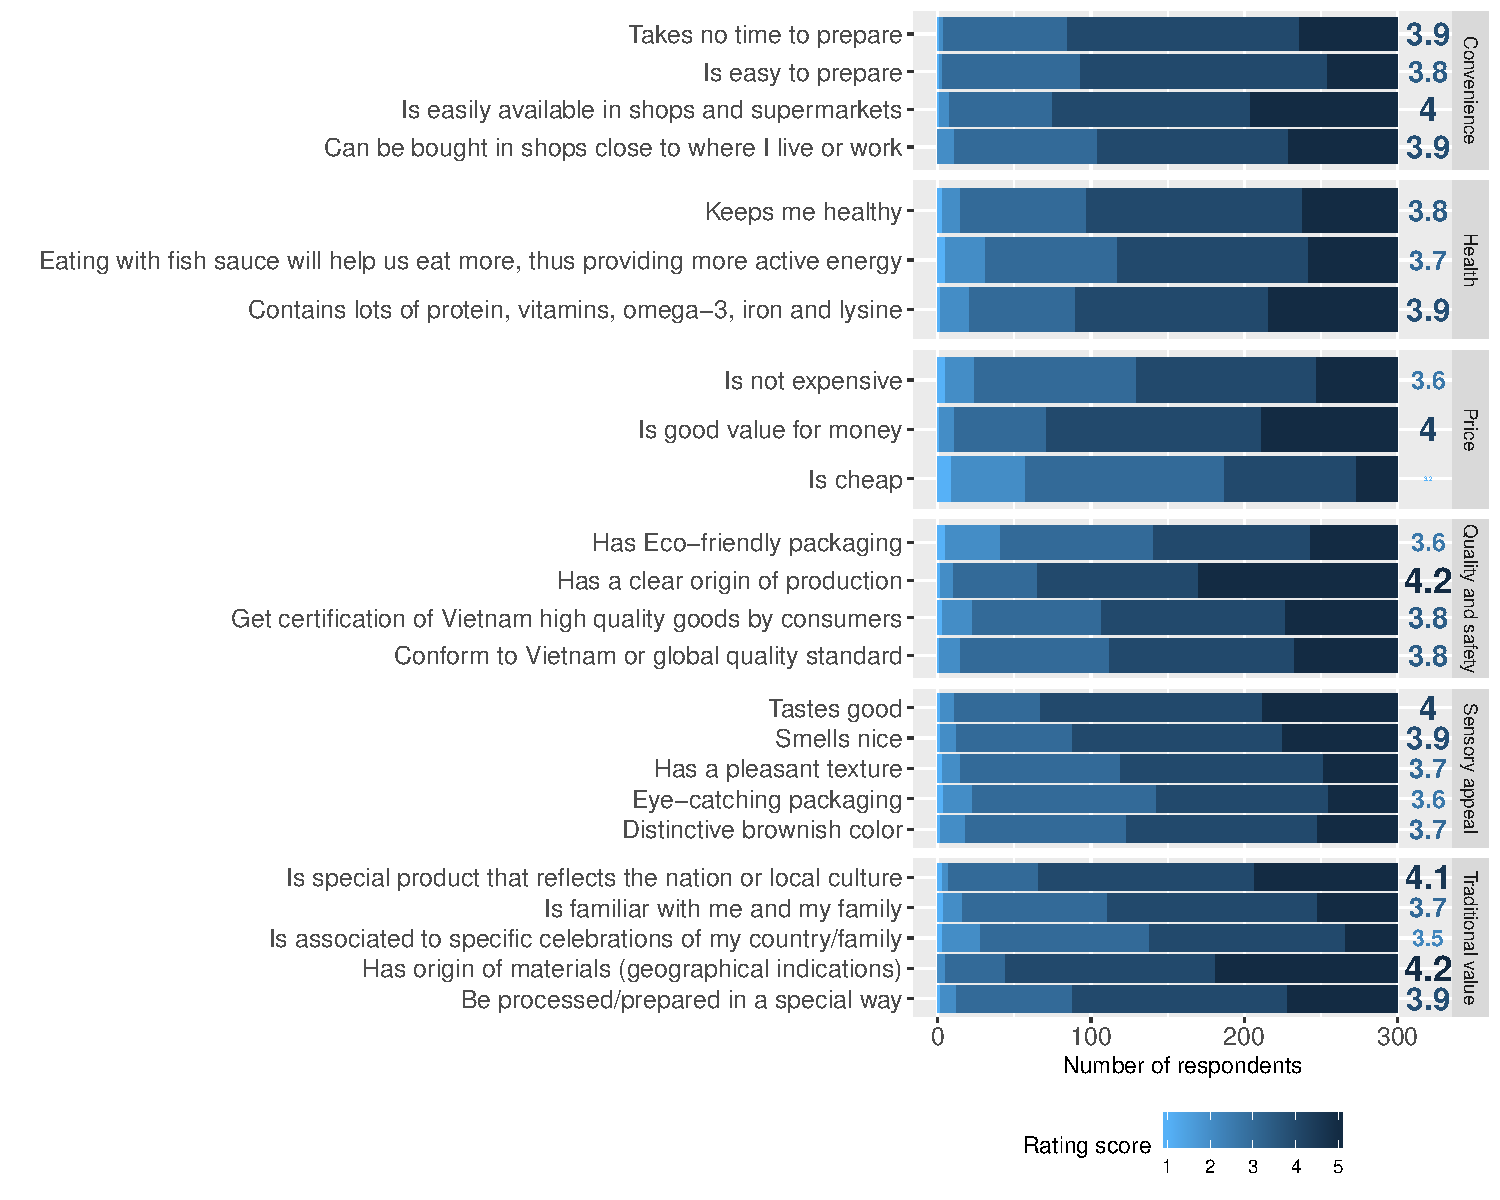
\includegraphics{Consumer-attitude-towards-fish-sauce-products_files/figure-latex/unnamed-chunk-15-1.pdf}

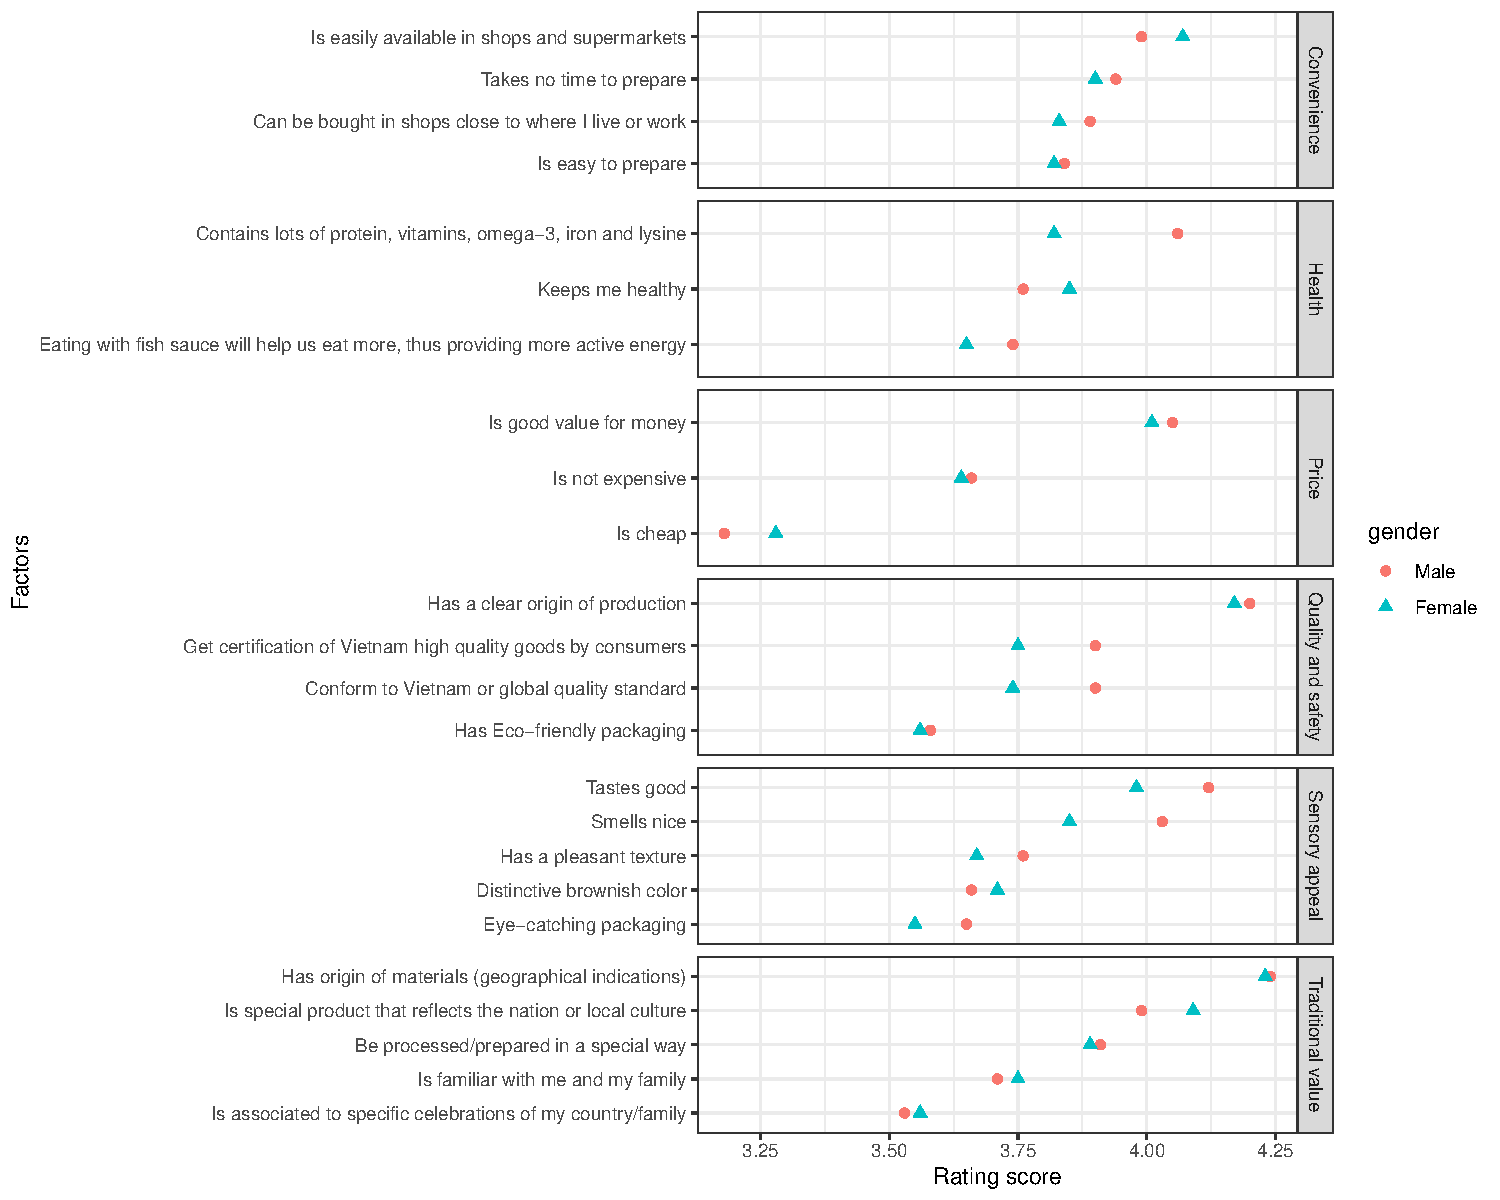
\includegraphics{Consumer-attitude-towards-fish-sauce-products_files/figure-latex/unnamed-chunk-16-1.pdf}


\end{document}
